\documentclass[12pt]{article}
\usepackage[utf8]{inputenc}
\usepackage[T2A]{fontenc}
\usepackage[russian,english]{babel}
\usepackage{amsmath,amsfonts,amssymb,euscript,graphicx,wrapfig,multirow}
\usepackage{dsfont}
\usepackage{amsthm}
\inputencoding{utf8}
\bibliographystyle{unsrt}
\textheight=240mm \textwidth=170mm
\hoffset=-17mm
\voffset=-17mm

\usepackage{hyperref}

\makeatletter
%\renewcommand{\fnum@figure}{Figure \thefigure}
\renewcommand{\@biblabel}[1]{#1.}
\makeatother

\theoremstyle{theorem}
\newtheorem{theorem}{Theorem}
\theoremstyle{dfn}
\newtheorem{dfn}{Definition}
\theoremstyle{remark}
\newtheorem{remark}{Remark}

\begin{document}
%\renewcommand\refname{\centering References}


% Переключаем язык на английский.
% Очень полезно как в плане типографики (в том числе расстановки переносов),
% так и в плане того, что не надо переименовывать "Рисунок" в "Figure"
\selectlanguage{english}


\begin{center}
\emph{Voronezh State University}
\end{center}

Avdeev N.N., Zvolinsky R.E., Momot E.A.

On particular diameter bounds for integral point sets in higher dimensions


\section{Introduction}



\begin{dfn}\label{dfn1}
	A planar integral point set (PIPS) is a set $\mathcal{P}$
	of non-collinear points in plane $\mathbb{R}^{2}$ such that
	for any pair of points $P_{1}, P_{2} \in \mathcal{P}$
	the Euclidean distance $|P_{1}P_{2}|$
	between points $P_{1}$ and $P_{2}$ is integral.
\end{dfn}

Definition \ref{dfn1} can be generalized as follows:

\begin{dfn}
	An integral point set $\mathcal{P}$ is a set of $n$ points in
	the $m$-dimensional Euclidean space $\mathbb{R}^{m}$ with pairwise
	integral distances.
\end{dfn}

How can we characterize an integral point set?
First of all, we can look at its dimension;
then, we can count the number of points in it, which is always finite~\cite{anning1945integral,erdos1945integral}
and is further called the cardinality;
finally, we can naturally% TODO: naturally/essentially? cf. arxiv/1
define the diameter of a finite point set.

\begin{dfn}
	A diameter of the integral point set $\mathcal{P}$ is defined as
	\begin{equation}
		\operatorname{diam(\mathcal{P})} = \underset{P_{1}, P_{2} \in
		\mathcal{P}}{\max} |P_{1}P_{2}|
	\end{equation}
\end{dfn}

Every integral point set also has a characteristic~\cite{kemnitz1988punktmengen,kurz2005characteristic}.

\begin{dfn}
	The function $d(m, n)$ is the minimum possible diameter of
	the integral point set $\mathcal{P}$ of $n$ points in
	$m$-dimensional Euclidean space $\mathbb{R}^{m}$.
\end{dfn}


%For a bit more sophisticated configurations, another functions are presented~\cite{kurz2008minimum,kreisel2008heptagon}.
%
%\begin{dfn}
%	The function $\overline{d}(m, n)$ is the minimum possible diameter of
%	the integral point set $\mathcal{P}$ of $n$ points in
%	$m$-dimensional Euclidean space $\mathbb{R}^{m}$
%	such that no $m+1$ points are located on an $(m-1)$-dimensional hyperplane.
%\end{dfn}

%\begin{dfn}
%	The function $\dot{d}(m, n)$ is the minimum possible diameter of
%	the integral point set $\mathcal{P}$ of $n$ points in
%	$m$-dimensional Euclidean space $\mathbb{R}^{m}$
%	such that no three points are located on a straight line
%	and no four points are located on a circle.
%\end{dfn}

For the list of known bounds for $d(m, n)$,
we refer the reader to~\cite[Theorem 1]{kurz2008bounds} or to~\cite{our-vmmsh-2018}.
We will discuss the following estimations presented at~\cite{kurz2008bounds}:
\begin{align}
	d(m, 2m + 1) \leq 8\\
	d(m, 2m + 2) \leq 13 \hypertarget{d2}\\
	d(m, 3m) \leq 109
\end{align}
and the following theorem \cite[Theorem 2.1]{kurz2008bounds}.

\begin{theorem}
	Let $\mathcal{P}$ be a planar integral point set consisting of
	$n - 2$ points on line $l$ and two points $P_{1}$ and $P_{2}$ on a
	parallel line $m$ with distance $r$ between $l_{1}$ and $l_{2}$. If there
	exist positive integers $v$, $w$ with $f^{2} + v^{2}
	= w^{2}$ and $v < 2r$, where $|P_{1}P_{2}| = f$,
	then

	\begin{equation}\label{formula1}
		d(m, n - 2 + 2(m - 2)) \leq \max(w, \operatorname{diam(\mathcal{P})})
	\end{equation}

\end{theorem}

Firstly, we discuss the classification of planar integral points sets;
then, we present some bounds for $d(m,n)$ based on planar integral point sets of particular types
and provide some general constructions for such bounds.

\section{Classification of planar integral point sets}

\subsection{Integral point sets situated in two straight lines}

\begin{dfn}
	A planar integral point sets of $n$ points with $n-1$ points on a straight line is called
	a \textit{facher} set.
\end{dfn}
Facher sets are very dominating examples of planar integral pont sets.
In~\cite{antonov2008maximal}, facher sets of characteristic 1 are called \textit{semi-crabs}.
For $9 \leq n \leq 122$, the diameter $d(2,n)$ is reached on a facher point set~\cite{kurz2008minimum}.

For non-facher integral point sets situated in two straight lines,
we can easily distinct the following three cases:

\begin{dfn}
	A planar integral point sets situated in two parallel straight lines
	is called a \textit{rails} set.
\end{dfn}

Among the rails sets, sets with 2 points on one line and all the other on another line dominate.

\begin{dfn}
	A planar integral point sets situated in two perpendicular straight lines
	is called a \textit{cross} set.
\end{dfn}
Every cross set has characteristic 1;
in~\cite{antonov2008maximal}, cross sets with only 2 points out of one of the lines are called \textit{crabs}.

\begin{dfn}
	A planar integral point sets situated in two straight lines
	that are not parallel nor perpendicular,
	is called a \textit{sciccors} set.
\end{dfn}

There is an important subclassof scissors sets.

\begin{dfn}
	A scissors set with an axis of symmetry,
	which is the angle bisector for the straight lines,
	is called a \textit{pyramid} set.
\end{dfn}

%TODO: rephrase?

%TODO: can a scissors set have another axis of symmetry?

\subsection{Other integral point sets}

\begin{dfn}
	A planar integral point sets that is situated on a circle is called a \textit{circular}
	point set.
\end{dfn}

Circular sets are very important examples
of integral point sets~\cite{harborth1993upper,piepmeyer1996maximum,bat2018number}.


\begin{dfn}
	A planar integral point sets that is situated on the conjunction of a circle with its center,
	is called a \textit{centered-circular} point set.
\end{dfn}

These six classes dominate among all the known planar integral point sets;
however, some sophisticated constructions are also known.

%TODO: pictures!

\section{Bounds based on rails sets}

Let $i = \overline{1, k}$ denote the enumeration of all $i$
from $1$ to $k$.
Theorem \cite[Theorem 2.1]{kurz2008bounds} can be generalized as follows:

\begin{theorem}
	Let $\mathcal{P}$ be a planar integral point set consisting of
	$n - k$ points on line $l_1$ and $k$ points $P_1$, $P_2$, ..., $P_k$ on a
	parallel line $l_2$ with distance $r$ between $l_1$ and $l_2$. If there
	exist positive integers $v$, $w_{ij}$, with $f_{ij}^{2} + v^{2}
	= w_{ij}^{2}$ and $v < 2r$, where $i = \overline{1, k - 1}$, $j =
	\overline{i + 1, k}$, $|P_{i}P_{j}| = f_{ij}$,
	then

	\begin{equation}
		d(m, n - k + k(m - k)) \leq \max(w_{1k}, \operatorname{diam(\mathcal{P})})
	\end{equation}

\end{theorem}

Below we give the planar integral point sets and the corresponding
estimates of the function $d(m, n)$ for $n = 2m + k$, $3 \leq k \leq 24$.
For convenience, we use the notation \cite{our-ped-2018,our-pmm-2018,our-vmmsh-2018}:
$\sqrt{p}/q * \{ (x_1,y_1), ...,$ $ (x_n, y_n)  \}$,
which means that each abscissa is multiplied by $1/q$
and each ordinate is multiplied by $\sqrt{p}/q$,  i.e.
$$
	\sqrt{p}/q * \{ (x_1,y_1), ..., (x_n, y_n)  \}
	=
	\left\{ \left(\frac{x_1}{q},\frac{y_1\sqrt{p}}{q}\right), ..., \left(\frac{x_n}{q},   \frac{y_n\sqrt{p}}{q}\right)  \right\}.
$$

\begin{itemize}
\setlength{\itemsep}{-1mm}


\begin{figure}[htbp]
	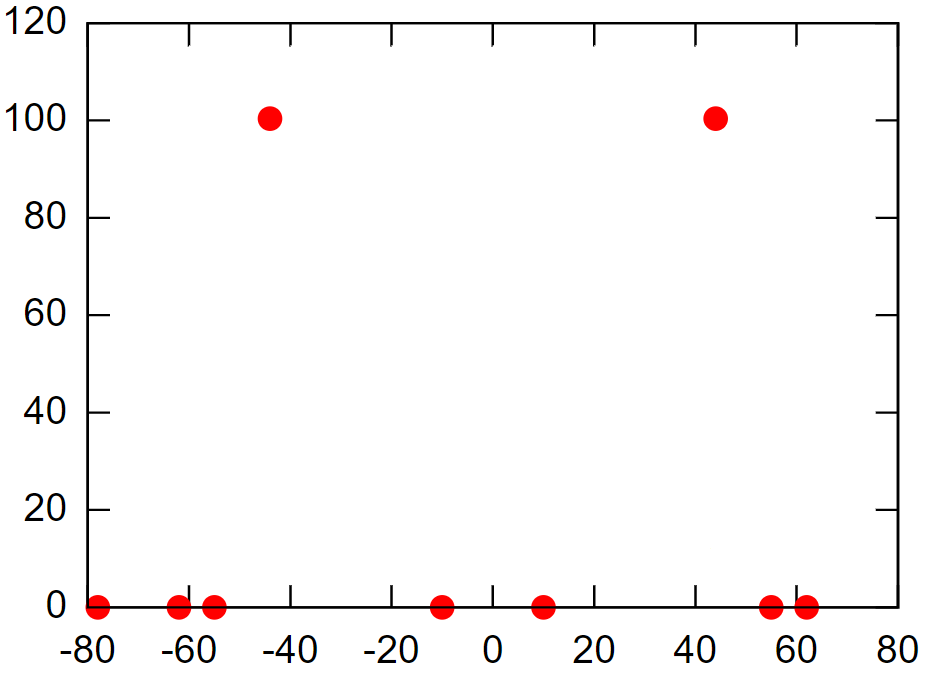
\includegraphics[width=.48\linewidth]{picture_2.png}
	\hfill
	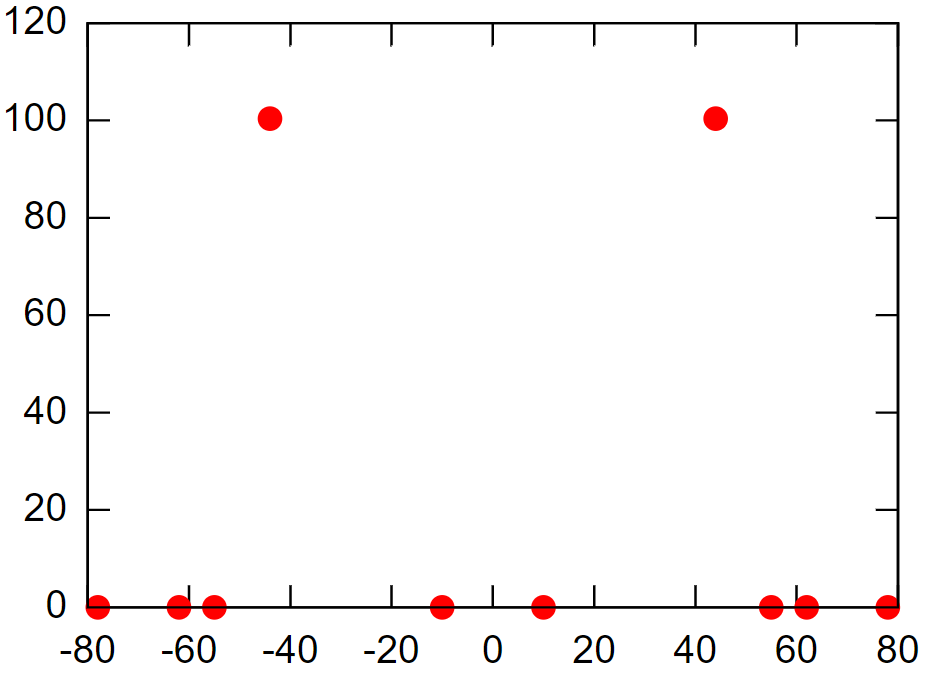
\includegraphics[width=.48\linewidth]{picture_3.png}
	\\
	\parbox{.48\linewidth}{\caption{PIPS of cardinality 9 and diameter 158}
	\label{picture_2.png}}
	\hfill
	\parbox{.48\linewidth}{\caption{PIPS of cardinality 10 and diameter 158}
	\label{picture_3.png}}
\end{figure}


\item
$\mathcal{P}=\sqrt{70}/{1} * \{ (\pm 44, 12),
(-78 , 0),
(\pm 62, 0),
(\pm 55 , 0),
(\pm 10 , 0)\}
$
(Figure~\ref{picture_2.png})

$f = 88$, $v = 66$, $w = 110$, $\operatorname{diam(\mathcal{P})} = 158$,

which gives $d(m, 2m + 3) \leq 158$.


\item
$\mathcal{P}=\sqrt{70}/{1} * \{ (\pm 44, 12),
(\pm 78 , 0),
(\pm 62, 0),
(\pm 55 , 0),
(\pm 10 , 0)\}
$
(Figure~\ref{picture_3.png}).

$f = 88$, $v = 66$, $w = 110$, $\operatorname{diam(\mathcal{P})} = 158$,

which gives $d(m, 2m + 4) \leq 158$.


\item
$\mathcal{P}=\sqrt{70}/{2} * \{ (\pm 99, 24),
(\pm 207 , 0),
(\pm 145 , 0),
(\pm 63 , 0),
(\pm 25 , 0),
(-297 , 0)\}
$
(Figure~\ref{picture_4.png}).

$f = 99$, $v = 20$, $w = 101$, $\operatorname{diam(\mathcal{P})} = 252$,

which gives $d(m, 2m + 5) \leq 252$.


\begin{figure}[htbp]
	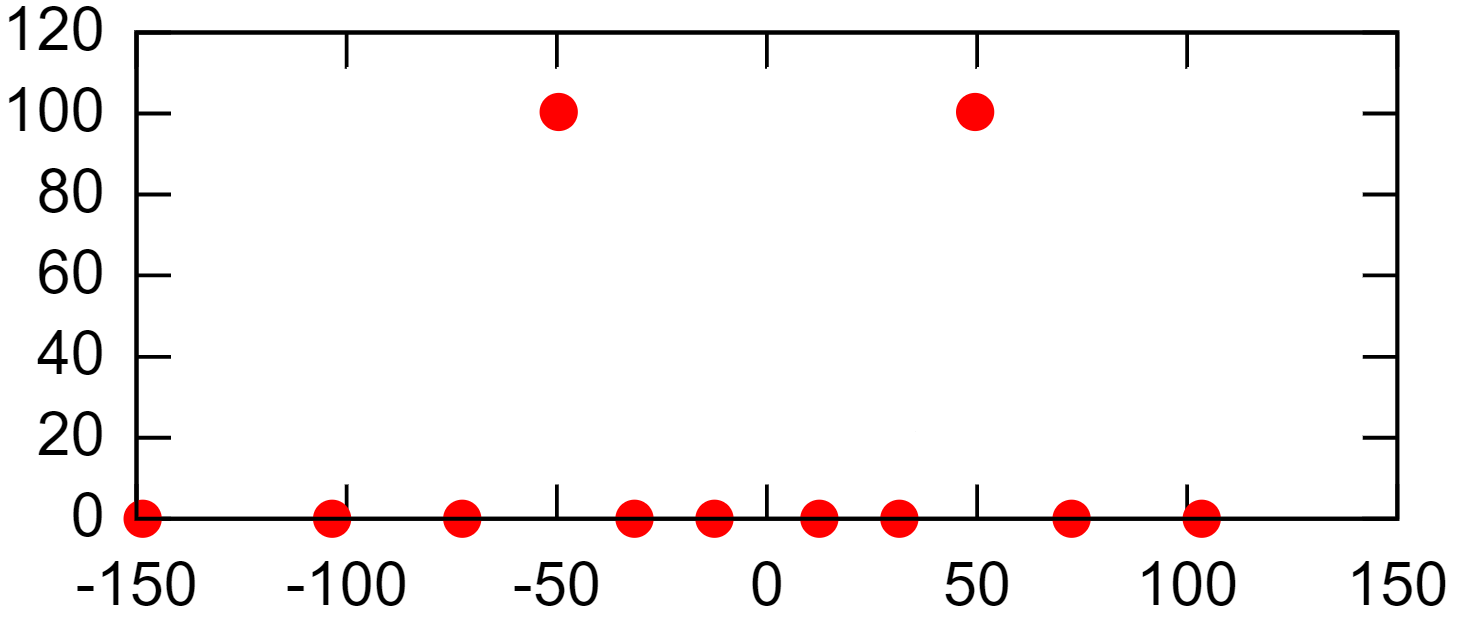
\includegraphics[width=.48\linewidth]{picture_4.png}
	\hfill
	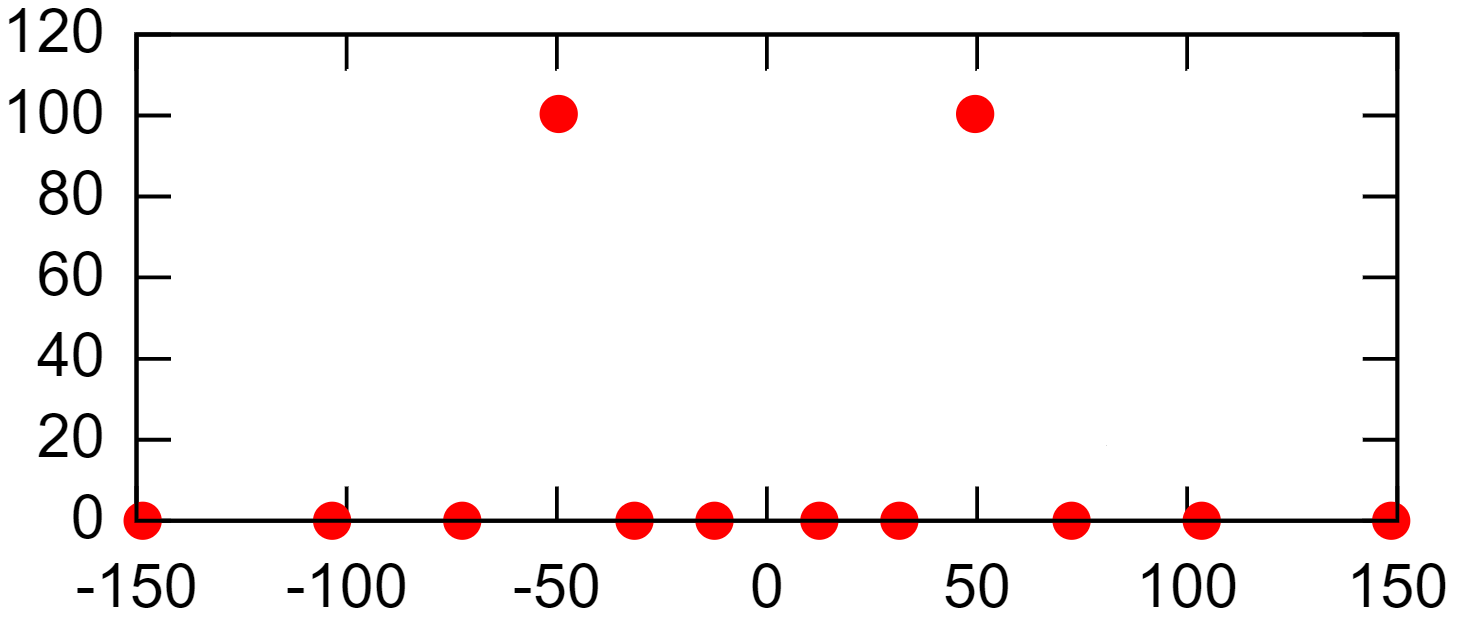
\includegraphics[width=.48\linewidth]{picture_5.png}
	\\
	\parbox{.48\linewidth}{\caption{PIPS of cardinality 11 and diameter 252}
	\label{picture_4.png}}
	\hfill
	\parbox{.48\linewidth}{\caption{PIPS of cardinality 12 and diameter 297}
	\label{picture_5.png}}
\end{figure}


\item
$\mathcal{P}=\sqrt{70}/{2} * \{ (\pm 99, 24),
(\pm 297 , 0),
(\pm 207 , 0),
(\pm 145 , 0),
(\pm 63 , 0),
(\pm 25 , 0)\}
$
(Figure~\ref{picture_5.png}).

$f = 99$, $v = 20$, $w = 101$, $\operatorname{diam(\mathcal{P})} = 297$,

which gives $d(m, 2m + 6) \leq 297$.


\item
$\mathcal{P}=\sqrt{19019}/{2} * \{ (\pm 200, 3),
(\pm 873 , 0),
(\pm 615 , 0),
(\pm 377 , 0),
(\pm 215 , 0),
(\pm 23 , 0),
$

$
(-1273 , 0)\}
$
(Figure~\ref{picture_6.png}).

$f = 200$, $v = 45$, $w = 205$, $\operatorname{diam(\mathcal{P})} = 1073$,

which gives $d(m, 2m + 7) \leq 1073$.


\begin{figure}[h!]
\center{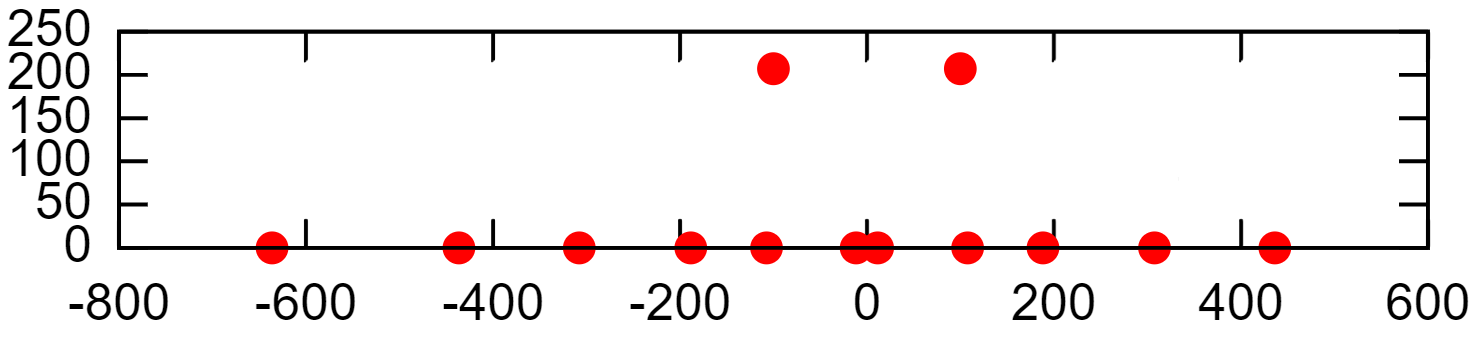
\includegraphics[width=0.7\linewidth]{picture_6.png}}
\parbox{0.7\linewidth}{\caption{IPS of cardinality 13 and diameter 1073}
\label{picture_6.png}}
\end{figure}


\item
$\mathcal{P}=\sqrt{19019}/{2} * \{ (\pm 200, 3),
(\pm 1273 , 0),
(\pm 873 , 0),
(\pm 615 , 0),
(\pm 377 , 0),
(\pm 215 , 0),
$

$
(\pm 23 , 0)\}
$
(Figure~\ref{picture_7.png}).

$f = 200$, $v = 45$, $w = 205$, $\operatorname{diam(\mathcal{P})} = 1273$,

which gives $d(m, 2m + 8) \leq 1273$.


\item
$\mathcal{P}=\sqrt{385}/{2} * \{ (\pm 1105, 48),
(\pm 1587 , 0),
(\pm 1269 , 0),
(\pm 763 , 0),
(\pm 623 , 0),
(\pm 529 , 0),
$

$
(\pm 339 , 0),
(-2189 , 0)\}
$
(Figure~\ref{picture_8.png}).

$f = 1105$, $v = 300$, $w = 1145$, $\operatorname{diam(\mathcal{P})} = 1888$,

which gives $d(m, 2m + 9) \leq 1888$.


\begin{figure}[h!]
\center{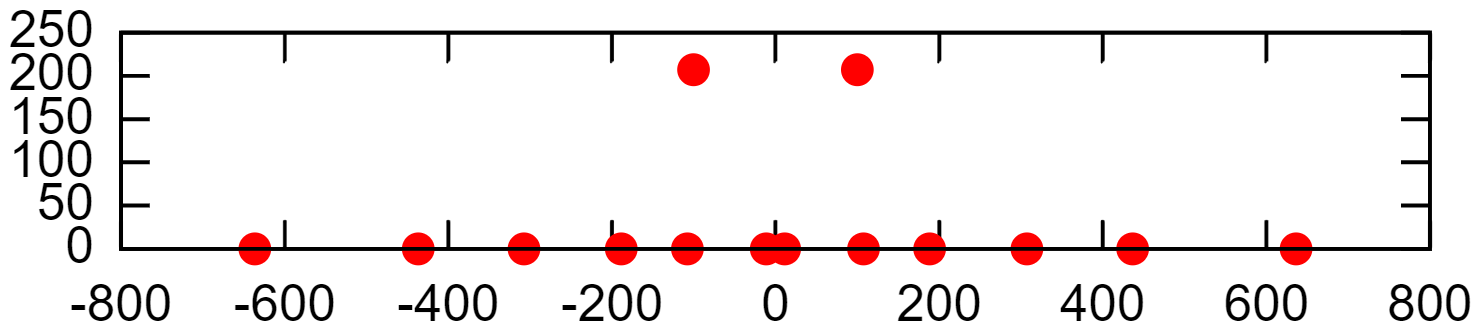
\includegraphics[width=0.7\linewidth]{picture_7.png}}
\parbox{0.7\linewidth}{\caption{IPS of cardinality 14 and diameter 1273}
\label{picture_7.png}}
\end{figure}


\begin{figure}[h!]
\center{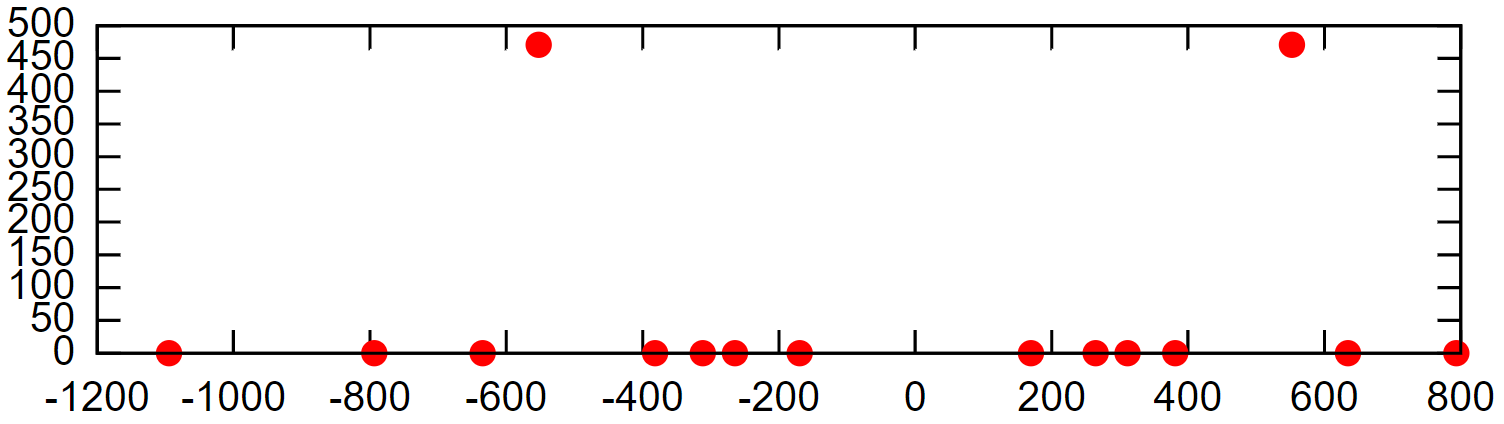
\includegraphics[width=0.75\linewidth]{picture_8.png}}
\parbox{0.75\linewidth}{\caption{IPS of cardinality 15 and diameter 1888}
\label{picture_8.png}}
\end{figure}


\item
$\mathcal{P}=\sqrt{385}/{2} * \{ (\pm 1105, 48),
(\pm 2189 , 0),
(\pm 1587 , 0),
(\pm 1269 , 0),
(\pm 763 , 0),
(\pm 623 , 0),
$

$
(\pm 529 , 0),
(\pm 339 , 0)\}
$
(Figure~\ref{picture_9.png}).

$f = 1105$, $v = 300$, $w = 1145$, $\operatorname{diam(\mathcal{P})} = 2189$,

which gives $d(m, 2m + 10) \leq 2189$.


\begin{figure}[h!]
\center{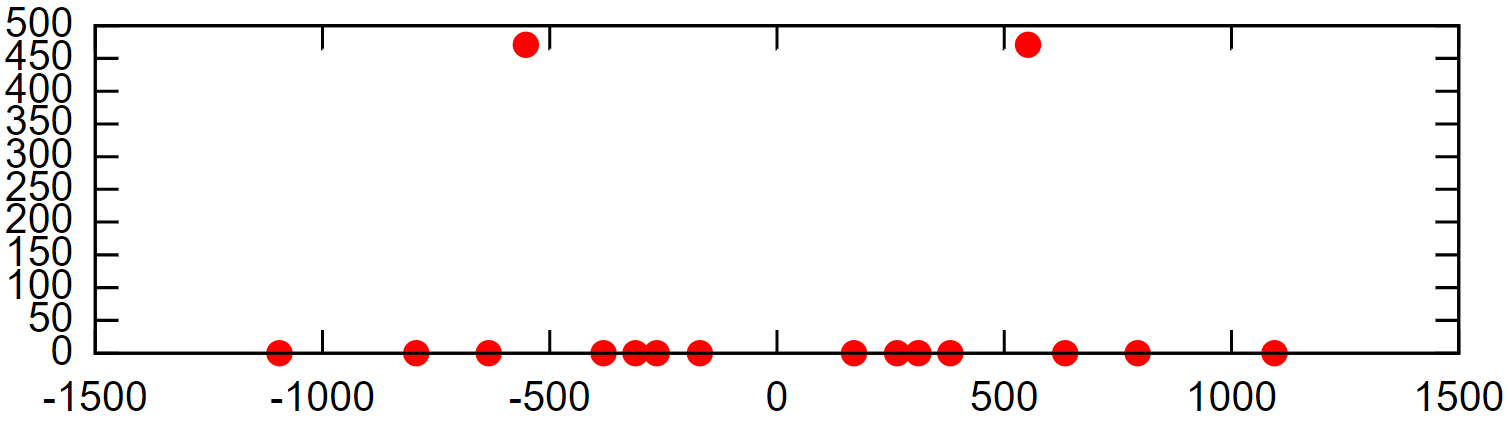
\includegraphics[width=0.75\linewidth]{picture_9.png}}
\parbox{0.75\linewidth}{\caption{IPS of cardinality 16 and diameter 2189}
\label{picture_9.png}}
\end{figure}


\item
$\mathcal{P}=\sqrt{154}/{1} * \{ (\pm 874, 60),
(\pm 1376 , 0),
(\pm 1036 , 0),
(\pm 899 , 0),
(\pm 849 , 0),
(\pm 613 , 0),
$

$
(\pm 576 , 0),
(\pm 100 , 0),
(-1848 , 0)\}
$
(Figure~\ref{picture_13.png}).

$f = 1748$, $v = 336$, $w = 1780$, $\operatorname{diam(\mathcal{P})} = 3224$,

which gives $d(m, 2m + 11) \leq 3224$.


\begin{figure}[h!]
\center{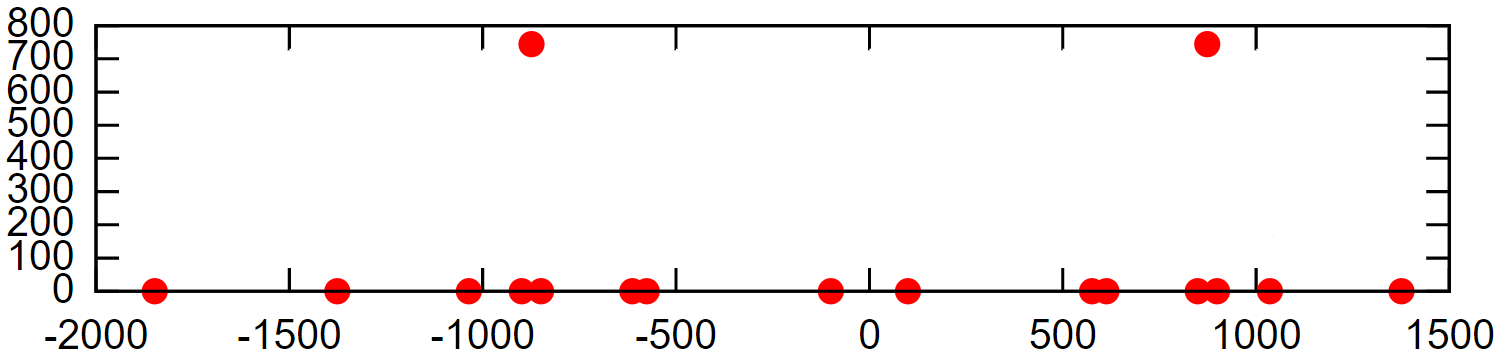
\includegraphics[width=0.85\linewidth]{picture_13.png}}
\parbox{0.85\linewidth}{\caption{IPS of cardinality 17 and diameter 3224}
\label{picture_13.png}}
\end{figure}


\item
$\mathcal{P}=\sqrt{154}/{1} * \{ (\pm 874, 60),
(\pm 1848 , 0),
(\pm 1376 , 0),
(\pm 1036 , 0),
(\pm 899 , 0),
(\pm 849 , 0),
$

$
(\pm 613 , 0),
(\pm 576 , 0),
(\pm 100 , 0)\}
$
(Figure~\ref{picture_14.png}).

$f = 1748$, $v = 336$, $w = 1780$, $\operatorname{diam(\mathcal{P})} = 3696$,

which gives $d(m, 2m + 12) \leq 3696$.


\begin{figure}[h!]
\center{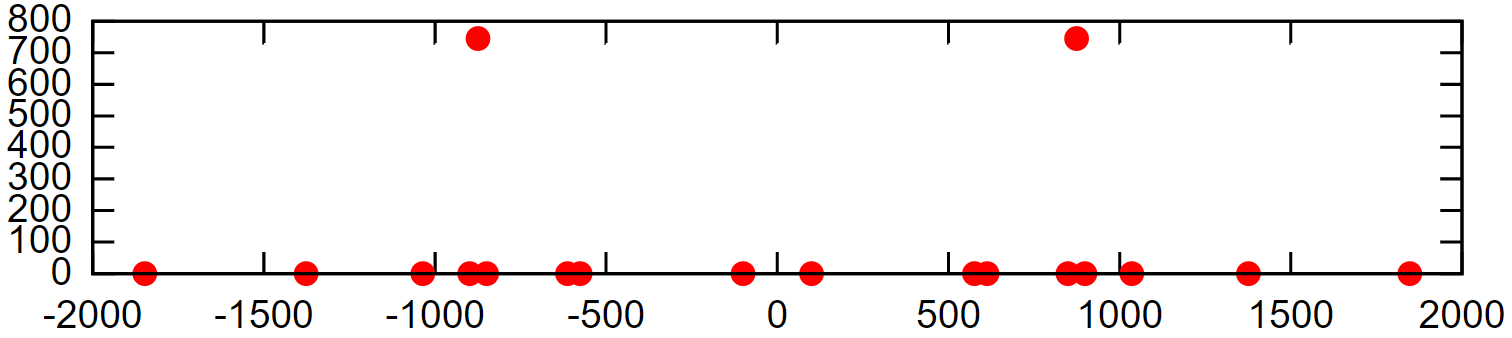
\includegraphics[width=0.85\linewidth]{picture_14.png}}
\parbox{0.85\linewidth}{\caption{IPS of cardinality 18 and diameter 3696}
\label{picture_14.png}}
\end{figure}


\item
$\mathcal{P}=\sqrt{154}/{1} * \{ (\pm 874, 60),
(\pm 1848 , 0),
(\pm 1376 , 0),
(\pm 1036 , 0),
(\pm 899 , 0),
(\pm 849 , 0),
$

$
(\pm 613 , 0),
(\pm 576 , 0),
(\pm 100 , 0),
(-3293 , 0)\}
$
(Figure~\ref{picture_15.png}).

$f = 1748$, $v = 336$, $w = 1780$, $\operatorname{diam(\mathcal{P})} = 5141$,

which gives $d(m, 2m + 13) \leq 5141$.


\begin{figure}[h!]
\center{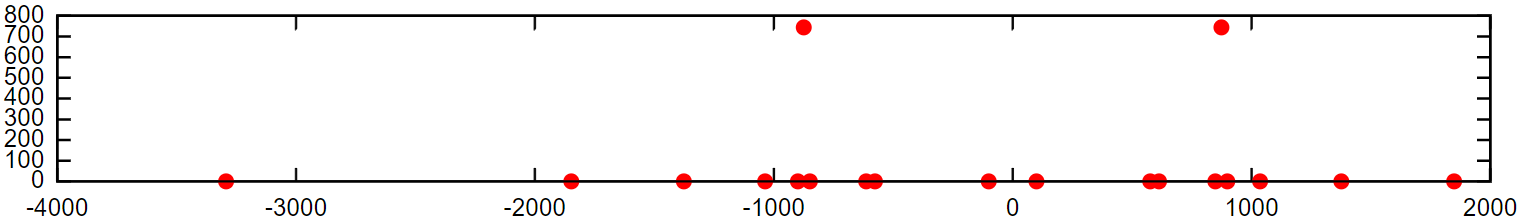
\includegraphics[width=1\linewidth]{picture_15.png}}
\parbox{1\linewidth}{\caption{IPS of cardinality 19 and diameter 5141}
\label{picture_15.png}}
\end{figure}


\item
$\mathcal{P}=\sqrt{154}/{1} * \{ (\pm 874, 60),
(\pm 3293 , 0),
(\pm 1848 , 0),
(\pm 1376 , 0),
(\pm 1036 , 0),
(\pm 899 , 0),
$

$
(\pm 849 , 0),
(\pm 613 , 0),
(\pm 576 , 0),
(\pm 100 , 0)\}
$
(Figure~\ref{picture_16.png}).

$f = 1748$, $v = 336$, $w = 1780$, $\operatorname{diam(\mathcal{P})} = 6586$,

which gives $d(m, 2m + 14) \leq 6586$.


\begin{figure}[h!]
\center{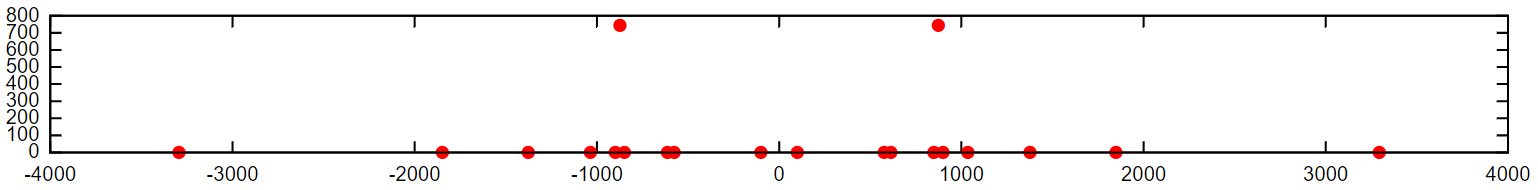
\includegraphics[width=1\linewidth]{picture_16.png}}
\parbox{1\linewidth}{\caption{IPS of cardinality 20 and diameter 6586}
\label{picture_16.png}}
\end{figure}


\item
$\mathcal{P}=\sqrt{154}/{1} * \{ (\pm 2622, 180),
(\pm 5544 , 0),
(\pm 4128 , 0),
(\pm 3108 , 0),
(\pm 2697 , 0),
$

$
(\pm 2547 , 0),
(\pm 1839 , 0),
(\pm 1728 , 0),
(\pm 904 , 0),
(\pm 300 , 0),
(-6148 , 0)\}
$
(Figure~\ref{picture_17.png}).

$f = 5244$, $v = 1008$, $w = 5340$, $\operatorname{diam(\mathcal{P})} = 11692$,

which gives $d(m, 2m + 15) \leq 11692$.


\item
$\mathcal{P}=\sqrt{154}/{1} * \{ (\pm 2622, 180),
(\pm 6148 , 0),
(\pm 5544 , 0),
(\pm 4128 , 0),
(\pm 3108 , 0),
$

$
(\pm 2697 , 0),
(\pm 2547 , 0),
(\pm 1839 , 0),
(\pm 1728 , 0),
(\pm 904 , 0),
(\pm 300 , 0)\}
$
(Figure~\ref{picture_18.png}).

$f = 5244$, $v = 1008$, $w = 5340$, $\operatorname{diam(\mathcal{P})} = 12296$,

which gives $d(m, 2m + 16) \leq 12296$.


\begin{figure}[h!]
\center{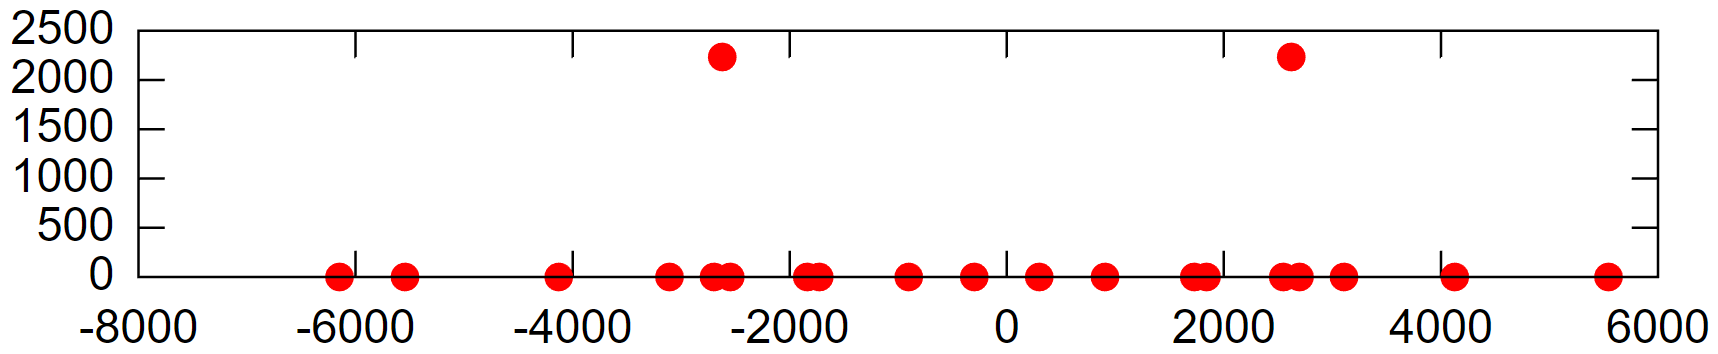
\includegraphics[width=0.75\linewidth]{picture_17.png}}
\parbox{0.75\linewidth}{\caption{IPS of cardinality 21 and diameter 11692}
\label{picture_17.png}}
\end{figure}


\item
$\mathcal{P}=\sqrt{154}/{1} * \{ (\pm 2622, 180),
(\pm 6148 , 0),
(\pm 5544 , 0),
(\pm 4128 , 0),
(\pm 3108 , 0),
$

$
(\pm 2697  , 0),
(\pm 2547 , 0),
(\pm 1839 , 0),
(\pm 1728 , 0),
(\pm 904 , 0),
(\pm 300 , 0),
(-9879 , 0)\}
$
(Figure~\ref{picture_19.png}).

$f = 5244$, $v = 1008$, $w = 5340$, $\operatorname{diam(\mathcal{P})} = 16027$,

which gives $d(m, 2m + 17) \leq 16027$.


\begin{figure}[h!]
\center{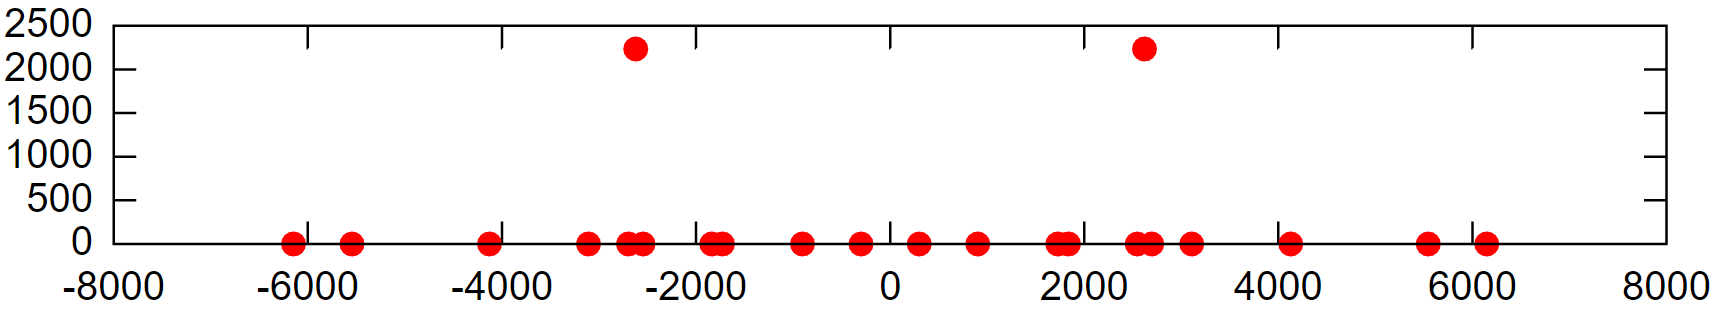
\includegraphics[width=0.75\linewidth]{picture_18.png}}
\parbox{0.75\linewidth}{\caption{IPS of cardinality 22 and diameter 12296}
\label{picture_18.png}}
\end{figure}


\item
$\mathcal{P}=\sqrt{154}/{1} * \{ (\pm 2622, 180),
(\pm 9879 , 0),
(\pm 6148 , 0),
(\pm 5544 , 0),
(\pm 4128 , 0),
$

$
(\pm 3108 , 0),
(\pm 2697 , 0),
(\pm 2547 , 0),
(\pm 1839 , 0),
(\pm 1728 , 0),
(\pm 904 , 0),
(\pm 300 , 0)\}
$
(Figure~\ref{picture_20.png}).

$f = 5244$, $v = 1008$, $w = 5340$, $\operatorname{diam(\mathcal{P})} = 19758$,

which gives $d(m, 2m + 18) \leq 19758$.


\begin{figure}[h!]
\center{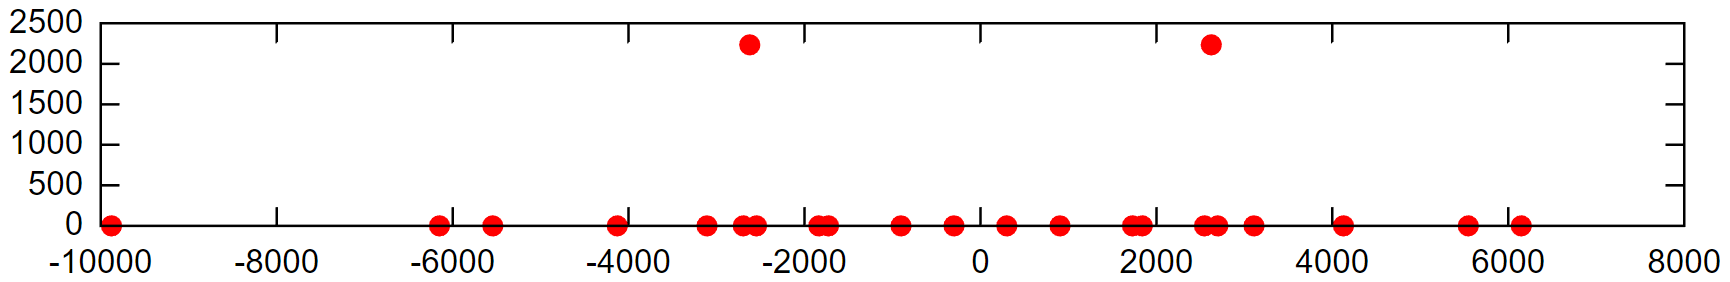
\includegraphics[width=0.85\linewidth]{picture_19.png}}
\parbox{0.85\linewidth}{\caption{IPS of cardinality 23 and diameter 16027}
\label{picture_19.png}}
\end{figure}


\item
$\mathcal{P}=\sqrt{154}/{1} * \{ (\pm 5244, 360),
(\pm 12296 , 0),
(\pm 11088 , 0),
(\pm 8579 , 0),
(\pm 8256 , 0),
$

$
(\pm 6216 , 0),
(\pm 5394 , 0),
(\pm 5094 , 0),
(\pm 3678 , 0),
(\pm 3456 , 0),
(\pm 1808 , 0),
(\pm 600 , 0),
$

$
(-19758 , 0)\}
$
(Figure~\ref{picture_21.png}).

$f = 10488$, $v = 1015$, $w = 10537$, $\operatorname{diam(\mathcal{P})} = 32054$,

which gives $d(m, 2m + 19) \leq 32054$.


\begin{figure}[h!]
\center{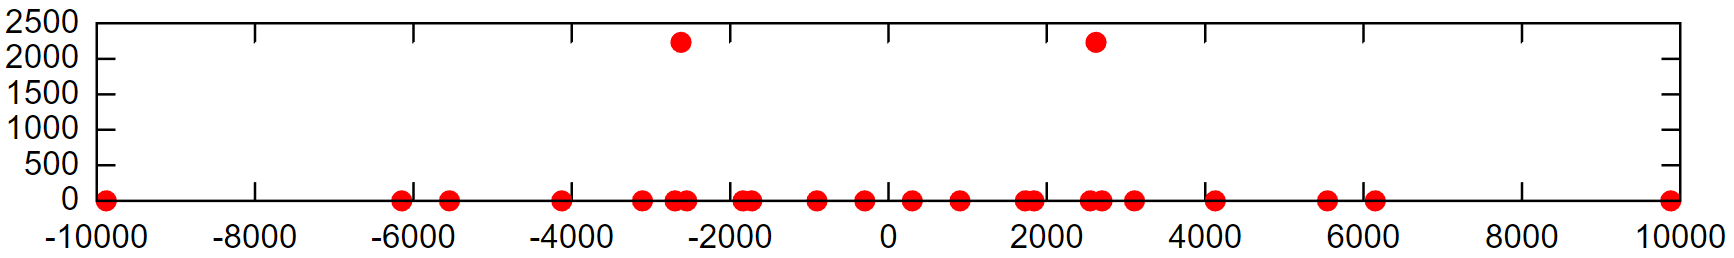
\includegraphics[width=0.85\linewidth]{picture_20.png}}
\parbox{0.85\linewidth}{\caption{IPS of cardinality 24 and diameter 19758}
\label{picture_20.png}}
\end{figure}


\begin{figure}[h!]
\center{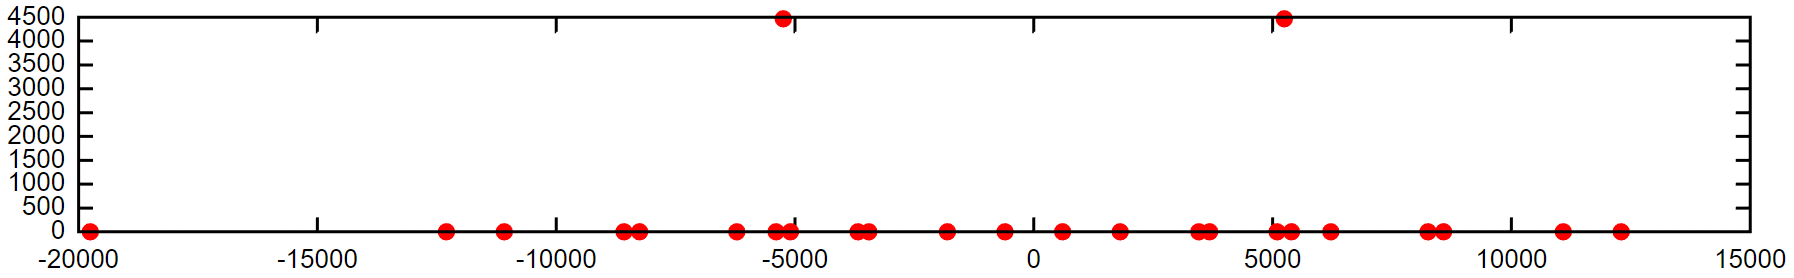
\includegraphics[width=1\linewidth]{picture_21.png}}
\parbox{1\linewidth}{\caption{IPS of cardinality 25 and diameter 32054}
\label{picture_21.png}}
\end{figure}


\item
$\mathcal{P}=\sqrt{154}/{1} * \{ (\pm 5244, 360),
(\pm 19758 , 0),
(\pm 12296 , 0),
(\pm 11088 , 0),
(\pm 8579 , 0),
$

$
(\pm 8256 , 0),
(\pm 6216 , 0),
(\pm 5394 , 0),
(\pm 5094 , 0),
(\pm 3678 , 0),
(\pm 3456 , 0),
(\pm 1808 , 0),
$

$
(\pm 600 , 0)\}
$
(Figure~\ref{picture_22.png}).

$f = 10488$, $v = 1015$, $w = 10537$, $\operatorname{diam(\mathcal{P})} = 39516$,

which gives $d(m, 2m + 20) \leq 39516$.


\begin{figure}[h!]
\center{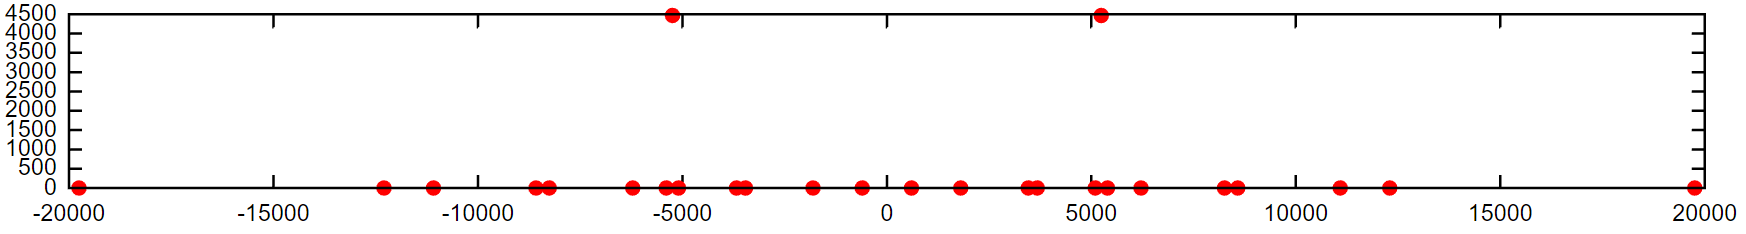
\includegraphics[width=1\linewidth]{picture_22.png}}
\parbox{1\linewidth}{\caption{IPS of cardinality 26 and diameter 39516}
\label{picture_22.png}}
\end{figure}


\item
$\mathcal{P}=\sqrt{154}/{1} * \{ (\pm 36708, 2520),
(\pm 116058 , 0),
(\pm 86072 , 0),
(\pm 77616 , 0),
(\pm 60053 , 0),
$

$
(\pm 57792 , 0),
(\pm 43512 , 0),
(\pm 37758 , 0),
(\pm 35658 , 0),
(\pm 25746 , 0),
(\pm 24192 , 0),
$

$
(\pm 12656 , 0),
(\pm 4200 , 0),
(-138306 , 0)\}
$
(Figure~\ref{picture_23.png}).

$f = 73416$, $v = 2710$, $w = 73466$, $\operatorname{diam(\mathcal{P})} = 254364$,

which gives $d(m, 2m + 21) \leq 254364$.


\begin{figure}[h!]
\center{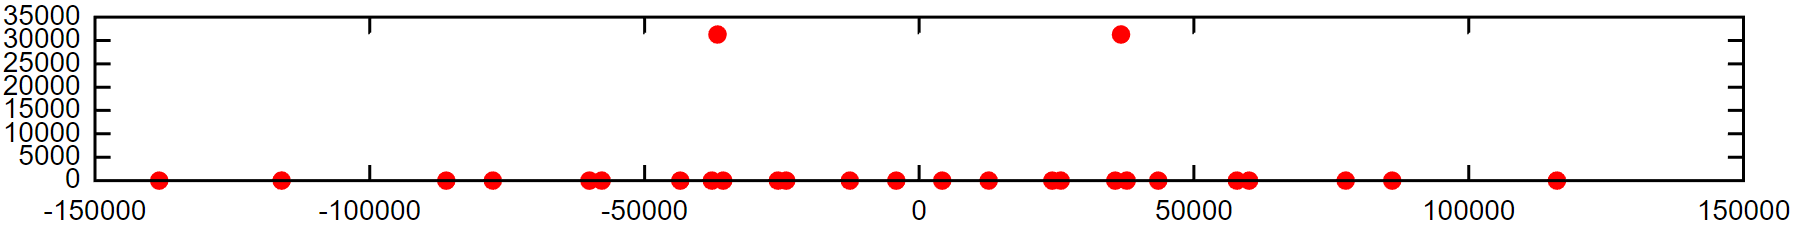
\includegraphics[width=1\linewidth]{picture_23.png}}
\parbox{1\linewidth}{\caption{IPS of cardinality 27 and diameter 254364}
\label{picture_23.png}}
\end{figure}


\item
$\mathcal{P}=\sqrt{154}/{1} * \{ (\pm 36708, 2520),
(\pm 138306 , 0),
(\pm 116058 , 0),
(\pm 86072 , 0),
(\pm 77616 , 0),
$

$
(\pm 60053 , 0),
(\pm 57792 , 0),
(\pm 43512 , 0),
(\pm 37758 , 0),
(\pm 35658 , 0),
(\pm 25746 , 0),
$

$
(\pm 24192 , 0),
(\pm 12656 , 0),
(\pm 4200 , 0)\}
$
(Figure~\ref{picture_24.png}).

$f = 73416$, $v = 2710$, $w = 73466$, $\operatorname{diam(\mathcal{P})} = 276612$,

which gives $d(m, 2m + 22) \leq 276612$.


\item
$\mathcal{P}=\sqrt{154}/{1} * \{ (\pm 36708, 2520),
(\pm 138306 , 0),
(\pm 116058 , 0),
(\pm 86072 , 0),
(\pm 77616 , 0),
$

$
(\pm 60053 , 0),
(\pm 57792 , 0),
(\pm 43512 , 0),
(\pm 37758 , 0),
(\pm 35658 , 0),
(\pm 25746 , 0),
$

$
(\pm 24192 , 0),
(\pm 12656 , 0),
(\pm 4200 , 0),
(-199863 , 0)\}
$
(Figure~\ref{picture_25.png}).

$f = 73416$, $v = 2710$, $w = 73466$, $\operatorname{diam(\mathcal{P})} = 338169$,

which gives $d(m, 2m + 23) \leq 338169$.


\begin{figure}[h!]
\center{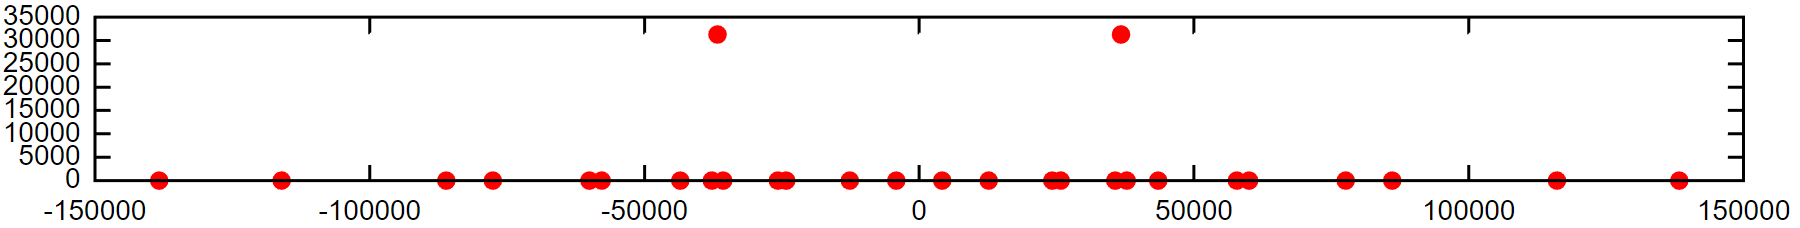
\includegraphics[width=1\linewidth]{picture_24.png}}
\parbox{1\linewidth}{\caption{IPS of cardinality 28 and diameter 276612}
\label{picture_24.png}}
\end{figure}


\begin{figure}[h!]
\center{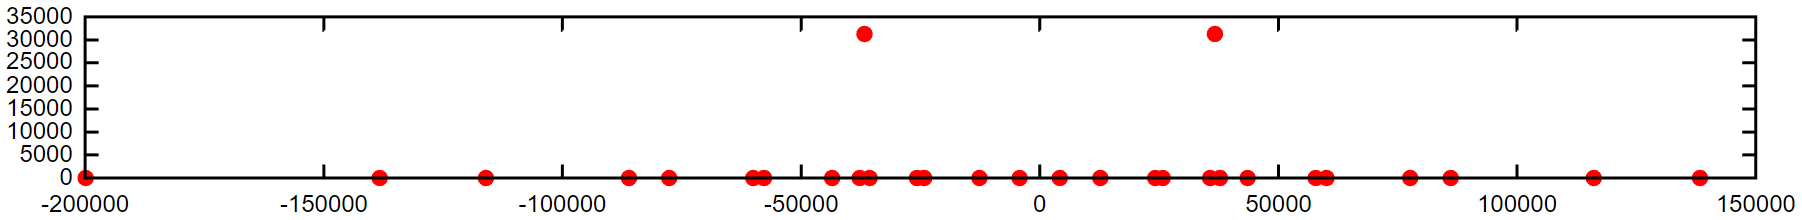
\includegraphics[width=1\linewidth]{picture_25.png}}
\parbox{1\linewidth}{\caption{IPS of cardinality 29 and diameter 338169}
\label{picture_25.png}}
\end{figure}


\item
$\mathcal{P}=\sqrt{154}/{1} * \{ (\pm 36708, 2520),
(\pm 199863 , 0),
(\pm 138306 , 0),
(\pm 116058 , 0),
(\pm 86072 , 0),
$

$
(\pm 77616 , 0),
(\pm 60053 , 0),
(\pm 57792 , 0),
(\pm 43512 , 0),
(\pm 37758 , 0),
(\pm 35658 , 0),
$

$
(\pm 25746 , 0),
(\pm 24192 , 0),
(\pm 12656 , 0),
(\pm 4200 , 0)\}
$
(Figure~\ref{picture_26.png}).

$f = 73416$, $v = 2710$, $w = 73466$, $\operatorname{diam(\mathcal{P})} = 399726$,

which gives $d(m, 2m + 24) \leq 399726$.


\begin{figure}[h!]
\center{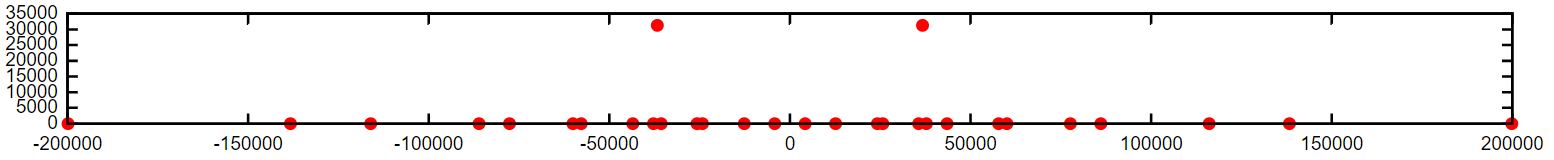
\includegraphics[width=1\linewidth]{picture_26.png}}
\parbox{1\linewidth}{\caption{IPS of cardinality 30 and diameter 399726}
\label{picture_26.png}}
\end{figure}


\end{itemize}

\begin{remark}
For all the examples above, maximum in the right part of (\ref{formula1})
evaluates to the diameter of the system.
The following example shows that the maximum can be evaluated to $w$:
\end{remark}


\begin{figure}[h!]
	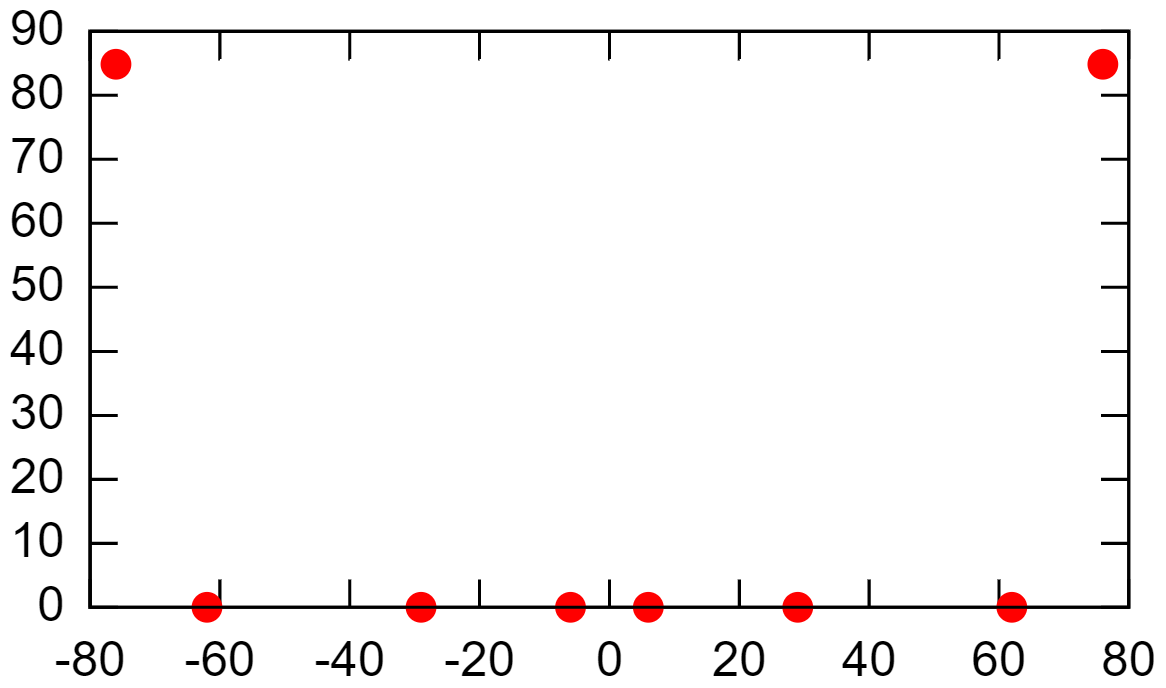
\includegraphics[width=.48\linewidth]{picture_10.png}
	\hfill
	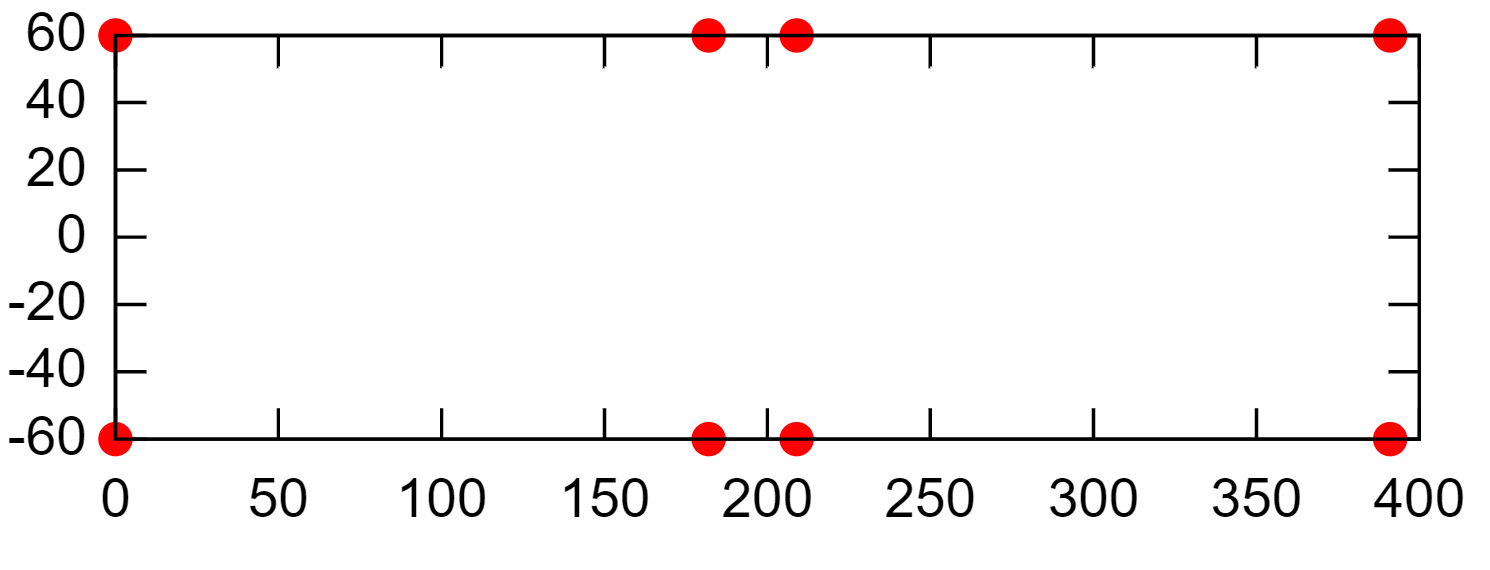
\includegraphics[width=.48\linewidth]{picture.png}
	\\
	\parbox{.48\linewidth}{\caption{PIPS of cardinality 8 and diameter 162}
	\label{picture_10.png}}
	\hfill
	\parbox{.48\linewidth}{\caption{PIPS of cardinality 8 and diameter 409}
	\label{picture.png}}
\end{figure}


\begin{itemize}
\setlength{\itemsep}{-1mm}


\item
$\mathcal{P}=\sqrt{2}/{1} * \{ (\pm 76, 60),
(\pm 62 , 0),
(\pm 29 , 0),
(\pm 6 , 0)\}
$
(Figure~\ref{picture_10.png}).

$f = 152$, $v = 114$, $w = 190$, $\operatorname{diam(\mathcal{P})} = 162$.

We can obtain the estimate $d(m, 2m + 2) \leq 190$ (which
is worse that known one (\hyperlink{d2}{2})).

\end{itemize}

Guy gives \cite[D 20]{guy2013unsolved} a system of $8$ points located
on two parallel lines. The points of the system form a rectangle
(Figure~\ref{rectangle.pdf}):

\begin{figure}[htbp]
	\includegraphics[width=.6\linewidth]{rectangle.pdf}
	\hfill
	\includegraphics[width=.5\linewidth]{right_angle.pdf}
	\\
	\parbox{.65\linewidth}{\caption{Distances}
	\label{rectangle.pdf}}
	\hfill
	\parbox{.5\linewidth}{\caption{Counterexample}
	\label{right_angle.pdf}}
\end{figure}

\begin{itemize}
\setlength{\itemsep}{-1mm}


\item
$\mathcal{P}=\sqrt{1}/{1} * \{ (0, \pm 60),
(182 , \pm 60),
(209 , \pm 60),
(391 , \pm 60)\}
$
(Figure~\ref{picture.png}),

where $n = 8$, $\operatorname{diam(\mathcal{P})} = 409$. Using the ``blowing up''
construction, we obtain
\begin{equation}\label{result1}
d(m, 4m) \leq 409
\end{equation}
Figure~\ref{picture_11.pdf} shows an example for $m = 3$.


\begin{figure}[h!]
\center{\includegraphics[width=1\linewidth]{picture_11.pdf}}
\parbox{1\linewidth}{\caption{IPS of cardinality 12 and diameter 409}
\label{picture_11.pdf}}
\end{figure}


\end{itemize}

\section{Bounds based on pyramid sets}

\begin{theorem}
Let $\mathcal{P}$ be a planar integral point set consisting of $k$
points on the line $l_{1}$ and $k$ points on the line $l_{2}$. Besides, these
points are symmetric with respect to one of the bisectors of the angles
formed by the intersection of lines $l_{1}$ and $l_{2}$, then

\begin{equation}\label{formula2}
d(m, (k - \alpha)m + \alpha) \leq \operatorname{diam(\mathcal{P})},
\end{equation}

where
\begin{equation*}
\alpha =
\begin{cases}
1, \text{when the intersection point} \in \mathcal{P}, \\
0, \text{when the intersection point} \notin \mathcal{P}.
\end{cases}
\end{equation*}

\end{theorem}

\begin{remark}
The angles can be acute or obtuse. Figure~\ref{right_angle.pdf} shows that the intersection angle of the lines $l_{1}$ and $l_{2}$ cannot be equal to ${\pi}/2$.
\end{remark}

Below we give the planar integral point sets and the corresponding
estimates of the function $d(m, n)$ for $n = 3m + 1$ and $n = 4m + 1$.

\begin{figure}[htbp]
	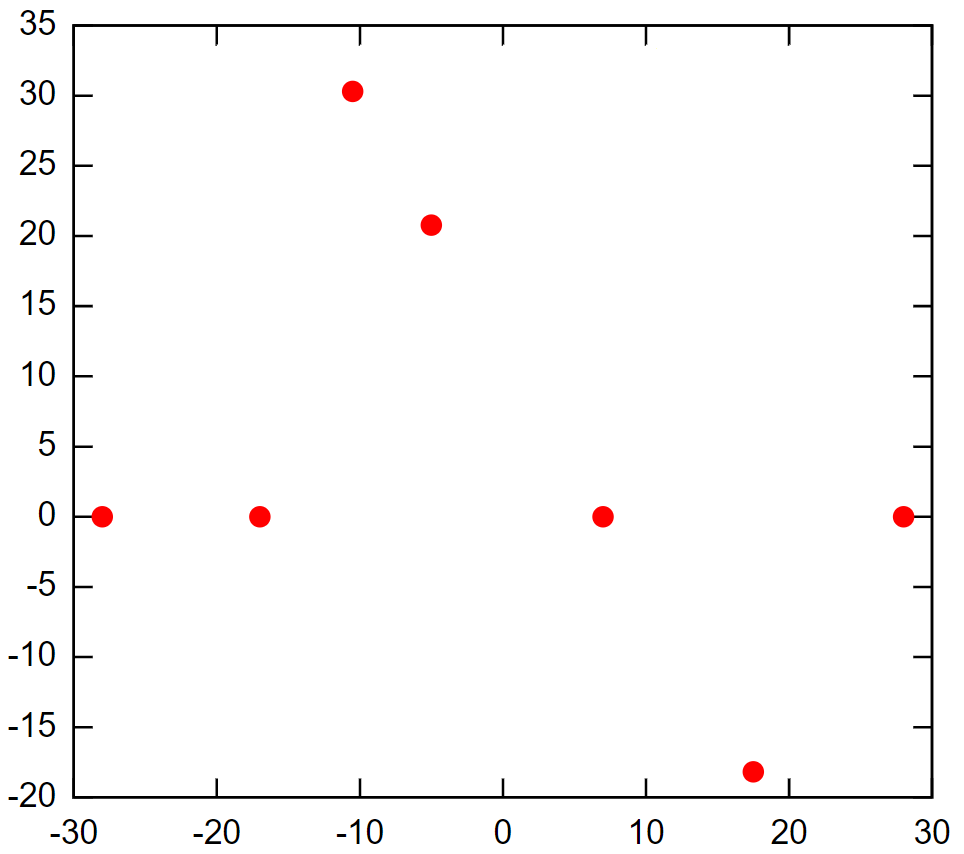
\includegraphics[width=.48\linewidth]{picture_56.png}
	\hfill
	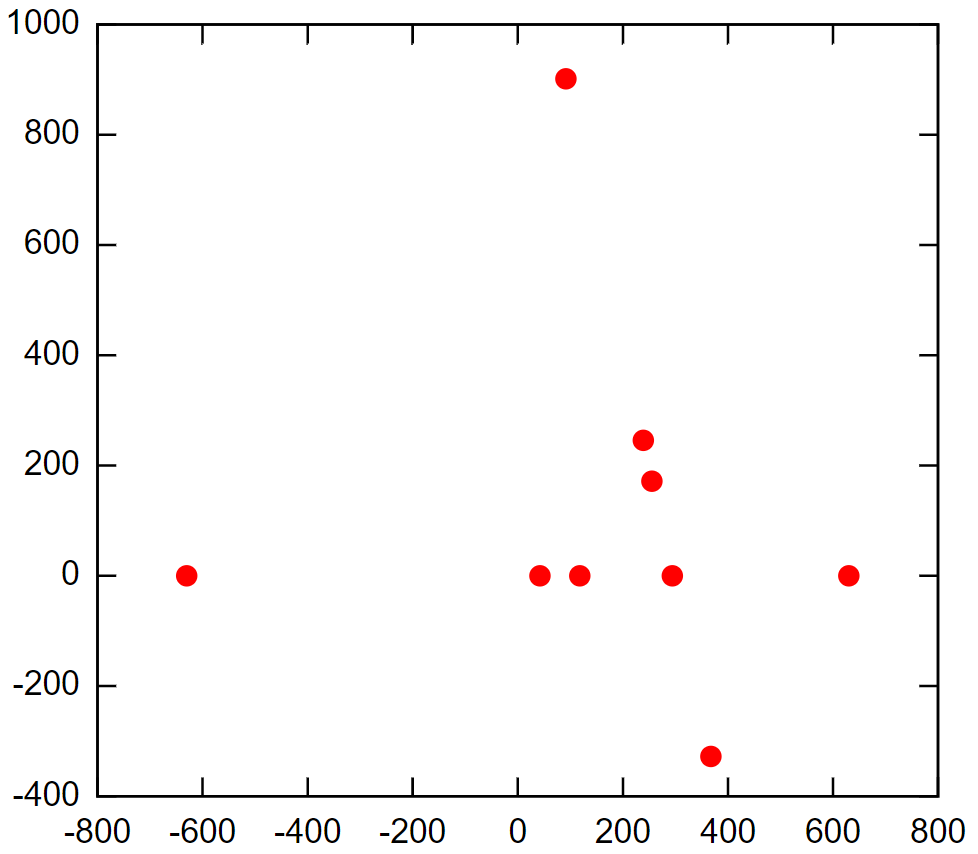
\includegraphics[width=.48\linewidth]{picture_1260.png}
	\\
	\parbox{.48\linewidth}{\caption{PIPS of cardinality 7 and diameter 56}
	\label{picture_56.png}}
	\hfill
	\parbox{.48\linewidth}{\caption{PIPS of cardinality 9 and diameter 1260}
	\label{picture_1260.png}}
\end{figure}

\begin{figure}[h!]
\center{\includegraphics[width=1\linewidth]{picture_12.pdf}}
\parbox{1\linewidth}{\caption{IPS of cardinality 10 and diameter 56}
\label{picture_12.pdf}}
\end{figure}

\begin{figure}[h!]
\center{\includegraphics[width=1\linewidth]{picture_1260_R3.pdf}}
\parbox{1\linewidth}{\caption{IPS of cardinality 13 and diameter 1260}
\label{picture_1260_R3.pdf}}
\end{figure}

\begin{itemize}
\setlength{\itemsep}{-1mm}


\item
$\mathcal{P}=\sqrt{3}/{2} * \{ (\pm 56, 0),
(14, 0),
(-34, 0),
(-10, 24),
(-21 , 35),
(35, -21)\}
$
(Figure~\ref{picture_56.png}),

where $n = 7$, $\operatorname{diam(\mathcal{P})} = 56$. Using the ``blowing up''
construction, we obtain
\begin{equation}\label{result2}
d(m, 3m + 1) \leq 56
\end{equation}
The resulting estimate improves the estimate for $d(m, 3m)$, which is presented
in \cite{kemnitz1988punktmengen}. Figure~\ref{picture_12.pdf} shows an example
for $m = 3$.


\item
$\mathcal{P}=\sqrt{39}/{8} * \{ (\pm 5040, 0),
(1911, 315),
(2352, 0),
(944, 0),
(336, 0),
(2940, -420),
(2044, 220),
$

$
(735, 1155)\}
$
(Figure~\ref{picture_1260.png}),

where $n = 9$, $\operatorname{diam(\mathcal{P})} = 1260$. Using the ``blowing up''
construction, we obtain
\begin{equation}\label{result3}
d(m, 4m + 1) \leq 1260
\end{equation}
Figure~\ref{picture_1260_R3.pdf} shows an example for $m = 3$.

\end{itemize}

\section{Final remarks}
All the given PIPSs were obtained through a combination of computer search an intuition of the authors;
so, the further search may lead to better bounds employing the same consructions.

There is still no general construction for a rails or scissors PIPS of given cardinality.
For rails PIPSs, we can conjecture that there exists a set of arbitrary cardinality with 2 points on one line
and all the rest on the other;
on the other hand, we still have not found any rails PIPSs with 4 and 5 points on the lines.

As for today, we have found pyramid PIPS of cardinality at most 9.

The source code can be obtained at https://gitlab.com/Nickkolok/ips-algo

\bibliography{literature}

\end{document}
